\chapter{HeidelTime and Its Multilingual Model} \label{the-chapter-3}
In this chapter, we give an overview of HeidelTime, discuss the data model of multilingual HeidelTime as presented by Str\"{o}tgen and Gertz in \cite{DBLP:conf/emnlp/StrotgenG15} and	 discuss some of its shortcomings.

\section{HeidelTime Overview}
HeidelTime is the first multilingual and domain-sensitive temporal tagger for the full task of temporal tagging \cite{DBLP:series/synthesis/2016Strotgen}. It has manually developed resources for 13 languages, and automatically developed resources for over 200 languages \cite{DBLP:conf/emnlp/StrotgenG15}. It is domain-sensitive, as in it can tag documents of differing domains such as news, narratives, scientific and colloquial \cite{DBLP:series/synthesis/2016Strotgen}. The online demo of HeidelTime can be accessed here\footnote{\url{http://heideltime.ifi.uni-heidelberg.de/heideltime/}}.

HeidelTime has been shown to perform very good in various competitions and corpora. It had best evaluation results for full task of temporal tagging for English in TempEval-2 \cite{DBLP:conf/semeval/VerhagenSCP10}, for English and Spanish in TempEval-3 \cite{DBLP:conf/semeval/UzZamanLDAVP13} and for Italian in Evalita 2014 \cite{caselli2014eventi}. In addition to the mentioned competitions, HeidelTime has been evaluated on various temporal corpora in languages such as Arabic, German, Chinese, among others\footnote{\url{https://github.com/HeidelTime/heideltime/wiki/Evaluation-Results}}. 

\subsection{Architecture}
HeidelTime's system architecture makes strict separation between algorithmic part (source code) and the resources part (patterns, rules and normalization information) \cite{DBLP:phd/de/Strotgen15}. The algorithmic core is language independent and written in Java, while the resources part is language dependent and written in .txt files arranged into three directories. One of HeidelTime's component called resource-interpreter, automatically loads the language dependent resources for tagging in the respective language if the resources are made in the format defined in \cite{DBLP:phd/de/Strotgen15}. This clear separation between algorithmic part and resources part in design of HeidelTime makes the manual extension to other languages appealing, which is evident from it being extended to languages such as German \cite{DBLP:phd/de/Strotgen15}, French \cite{moriceau2013french} and Croatian \cite{skukan2014heideltime}. 

\subsection{Availability}
HeidelTime is available as a standalone version and as a UIMA (Unstructured Information Management Architecture) kit (download link\footnote{\url{https://github.com/HeidelTime/heideltime/releases}}). The standalone version can be used in simpler cases; for instance, if only tagging is desired. The UIMA version of HeidelTime can be used in more advanced cases; for instance, to reproduce evaluation results. Apache UIMA\footnote{\url{https://uima.apache.org/}} is a Java framework that enables applications to be decomposed into components and use such components in a pipeline fashion. UIMA also defines a format called CAS (Common Analysis Structure), and all components in the pipeline work on CAS objects. As HeidelTime requires text to be pre-annotated with some preprocessing steps such tokenization, sentence splitting and part-of-speech tagging; and UIMA framework supports the idea of components in a pipelined fashion, HeidelTime was developed as a UIMA analysis engine component \cite{DBLP:phd/de/Strotgen15}. 

Some components bundled with HeidelTime UIMA version include: TempEval-2 Reader, a \ul{UIMA collection reader}, reads TempEval-2 annotated corpora and creates a CAS object for each document \cite{DBLP:phd/de/Strotgen15}. Heideltime, available as a \ul{UIMA analysis engine}, tags the documents temporally using TIMEX3 tags \cite{DBLP:phd/de/Strotgen15}. TempEval-3 Writer, a \ul{UIMA CAS consumer}, outputs temporally tagged documents in a format that official TempEval-3 evaluation scripts can run on \cite{DBLP:phd/de/Strotgen15}. The components to do preprocessing tasks such as tokenization, sentence splitting and part-of-speech tagging are also available with the HeidelTime kit as UIMA analysis engine components, and should be run before running the HeidelTime analysis engine component. 

\subsection{Resources}
For each language, HeidelTime arranges the resources into three directories, i.e., pattern resources, normalization resources and rule resources \cite{DBLP:phd/de/Strotgen15}. These directories hold .txt files, that have patterns, normalization and rules in them respectively.  

\textbf{Pattern Resources}\\
The pattern resources hold regular expressions for various kinds of temporal expressions such as month names, weekday names, etc. These .txt pattern files hold one regular expression on each line for legibility. The HeidelTime resource interpreter reads a pattern file and makes complete regular expression for respective pattern file automatically \cite{DBLP:phd/de/Strotgen15}. For instance, one of the file in pattern directory is called ``reMonthName", and for English language this file will hold the regular expressions for month names in English, i.e., [Jj]anuary, [Ff]ebruary, and so on in it. Similarly, for Urdu language it will have the month names \texturdu{جنوری}, \texturdu{فروری}, \texturdu{مارچ} and so on in it. 

Following listing depicts a part of a reMonthName for French language. \\

%\begin{figure}[H]
%	\centering
%	\includegraphics[width=8cm]{fr-reMonthName}
%	\caption{reMonthName - a sample French pattern resource for HeidelTime}
%	\label{figure:3a}
%\end{figure}

\begin{minipage}{\linewidth}
\lstset{caption={reMonthName - a sample French pattern resource for HeidelTime.}, label={listing:3-fr-reMonthName},}
\begin{lstlisting}
// english: January, 01
[Jj]anvier
// english: February, 02
[Ff]évrier
// english: March, 03
[Mm]ars
// english: April, 04
[Aa]vril
// english: May, 05
// ...
\end{lstlisting}
\end{minipage}

\textbf{Normalization Resources}\\
The normalization resources hold the temporal expression regular expressions and their normalized expressions separated by a comma, like a key-value pair. Like pattern .txt files, the normalization .txt files also hold one normalization information on each line. The HeidelTime resource interpreter reads a normalization file and holds the normalization information, so it can be used to assign normalized values to extracted temporal expressions. For instance, the first line in ``normMonthName" resource file for English can be \framebox{``[Jj]anuary",``01"} and the first line for Urdu can be \framebox{``\texturdu{جنوری}",``01"}

Following listing depicts a part of a normMonthName for French language. \\


%\begin{figure}[H]
%	\centering
%	\includegraphics[width=8cm]{fr-normMonthName}
%	\caption{normMonthName - a sample French normalization resource for HeidelTime}
%	\label{figure:3b}
%\end{figure}

%\begin{lstlisting}[
%caption={normMonthName - a sample French normalization resource for HeidelTime}, label={listing:3-fr-normMonthName}
%identifierstyle=\oddtest,
%commentstyle=\oddtest,
%stringstyle=\oddtest,
%keywordstyle=\oddtest,
%linebackgroundcolor={\ifodd\value{lstnumber}\color{cream}\fi}
%]
%... alternating , rows, colors
%... zebra color effect 
%\end{lstlisting}

\begin{minipage}{\linewidth}
\lstset{caption={normMonthName - a sample French normalization resource for HeidelTime.}, label={listing:3-fr-normMonthName},}
\begin{lstlisting}
// english: January, 01
"[Jj]anvier","01"
// english: February, 02
"[Ff]évrier","02"
// english: March, 03
"[Mm]ars","03"
// english: April, 04
"[Aa]vril","04"
// english: May, 05
// ...
\end{lstlisting}
\end{minipage}




\textbf{Rule Resources}\\
The rule resources hold the rules that are used to extract and normalize the temporal expressions from the text \cite{DBLP:phd/de/Strotgen15}. The rules extraction part make use of the pattern resources, and rules normalization part make use of the normalization resources. Like pattern and normalization resources, the rules are also read by HeidelTime's resource interpreter and made use of by its algorithmic part. HeidelTime defines a well-defined rule syntax to be used in the rule resources \cite{DBLP:phd/de/Strotgen15}. 

Each HeidelTime rule should have three obligatory parts, i.e., RULENAME, EXTRACTION and NORM\_VALUE. The RULENAME is helpful for statistics purposes, EXTRACTION part is used for extraction and here the names of pattern resources can be used to describe the regular expression to match, and NORMALIZATION part is used for normalization and here the names of normalization resources can be used \cite{DBLP:phd/de/Strotgen15}. In addition, rules may use some other parts such as specifying part-of-speech type of the token to extract. 

%We illustrate the rule syntax using a simple rule below, and for details refer the reader to Section 3.5.4 of \cite{DBLP:phd/de/Strotgen15}.

%\begin{figure}[H]
%	\centering
%	\includegraphics[width=14cm]{daterules}
%	\caption{rules\_daterules - a sample rule resource for HeidelTime}
%	\label{figure:3c}
%\end{figure}

Following listing shows a part of language independent rules resource of HeidelTime, that has some date rules in it.  \\

\begin{minipage}{\linewidth}
\begin{lstlisting}[caption={rules\_daterules - a sample rule resource for HeidelTime.}, label={listing:3-daterules}]
// r3a: March 30, 2000
// r3b: March 30

RULENAME="date_r3a",EXTRACTION="%reMonthName %reDayNumber,? %reYear4Digit",NORM_VALUE="group(3)-%normMonthName(group(1))-%normDayNumber(group(2))"

RULENAME="date_r3b",EXTRACTION="%reMonthName %reDayNumber",NORM_VALUE="UNDEF-year-%normMonthName(group(1))-%normDayNumber(group(2))"
// ...
\end{lstlisting}
\end{minipage}


In Listing \ref{listing:3-daterules}, some of the date rules are given. For instance, the rule named ``date\_3a" can extract dates such as \framebox{March 30, 2000} or \framebox{February 10 2012}. This can be gathered from the extraction part of the rule. We can see that the extraction part of the rule uses the pattern resources, by appending \% in front of the pattern resource name. Writing \%reMonthName will get all the month name patterns from the reMonthName pattern resource of a respective language. Following \%reMonthName is a space, then \%reDayNumber that refers to all patterns of day numbers from 1-31, then there is an optional comma, and finally the pattern \%reYear4Digit. 

In normalization part of the rule ``date\_3a", we see the normalized value that should be assigned to the extracted temporal expression. The first thing to notice is group(3); in HeidelTime each pattern in the extraction part counts as a group()-function, in addition to the patterns specified in parenthesis \cite{DBLP:phd/de/Strotgen15}. So in the order the pattern resource names appear in extraction part of rule, we can learn that \%reMonthName can be referred to as group(1), \%reDayNumber can be referred to as group(2) and \%reYear4Digit can be referred to as group(3) in the normalization part of the rule. Furthermore we can see, the group(1) and group(2) are enclosed in respective normalization functions, because reMonthName and reDayNumber will require normalization, unlike reYear4Digit. Thus, the normalization part is normalizing the extracted date to the ISO format (Table \ref{table:1a} page \pageref{table:1a}).

For a detailed overview of HeidelTime's rule syntax, we refer the reader to Section 3.5.4 of \cite{DBLP:phd/de/Strotgen15}.

\section{Multilingual HeidelTime Model} \label{multilingual-ht-model}
HeidelTime was extended to support over 200 languages using automatically developed resources by Str\"{o}tgen and Gertz in \cite{DBLP:conf/emnlp/StrotgenG15}. 

Now that we are familiar with the separation of algorithmic part and resources part in HeidelTime. We can understand that no changes to algorithmic part were required to support additional languages. Only the development of resources part of over 200 languages was to be done in order to make HeidelTime work in that many languages. Turning our attention to the resources part, we know that there are three kinds of resources in HeidelTime as already mentioned, i.e., pattern, normalization and rules. To create automatically developed resources for each language, the authors started with some initial resources. 

\subsection{Initial Resources} \label{res-ir}
The initial resources are a starting point, that are used to create the resources for each language . The authors in \cite{DBLP:conf/emnlp/StrotgenG15}, divided the initial resources in three categories. 

\begin{enumerate}[i.]
	\item \textbf{Language Dependent Resources:} \label{res-ir-i} These are written as simplified English normalization resources, and are used to make pattern and normalization resources for each language \cite{DBLP:conf/emnlp/StrotgenG15}. These resources are also called \ul{English-to-translate} resources, because they are used to make the actual language dependent resources of respective languages.  For instance, few such resources are: normMonthName that has normalization information such as \framebox{``January",``01"}, \framebox{``February",``02"} and so on in it, normDayNumberWord that has normalization information such as  \framebox{``one",``01"}, \framebox{``two",``02"} and so on in it.  
	
	\item \textbf{Language Independent Resources:}  These are written as pattern and normalization resources, and added as they are to the final resources for each language. For instance, two such resources are: a pattern resource reYear2Digit that has the regular expression \framebox{\textbackslash{}d\textbackslash{}d} in it and shall be used by all languages, and a normalization resource normMonthInSeason that has normalization information such as \framebox{``01",``WI"}, \framebox{``02",``WI"}, \framebox{``03",``SP"} and so on in it and shall also be used by all languages. 
	
	\item \textbf{Language Independent Rules:} \label{res-lir} These are the rules that are used by each language and are language independent. These rules are added as they are to the final resources of each language. Several orderings of patterns are used as different languages have different orderings in which the patterns appear. For instance, different orderings allow to extract both temporal expressions like ``20th April" and ``April 20th" \cite{DBLP:conf/emnlp/StrotgenG15}. 
\end{enumerate}

\subsection{Creating Final Resources}
To create the final resources, the initial resources mentioned before, are used. The first step is to create respective pattern and normalization resources for each of the language using the language dependent resources, albeit the created resources for all languages are empty at the moment. The second step is to extract patterns from the language dependent resources, and in third step these patterns are used to get translations for various languages from Wiktionary\footnote{\url{https://www.wiktionary.org/}}. The fourth step is to fill the pattern and normalization resources for all languages that were created in the first step. Once this is done, the process of creating automatically developed resources is almost complete. Finally, the language independent resources and language independent rules are added into the newly created resources of each language to get the final automatically developed resources \cite{DBLP:conf/emnlp/StrotgenG15}.

An overview of automated resource development process is given in the figure below:  
\begin{figure}[H] 
	\centering
	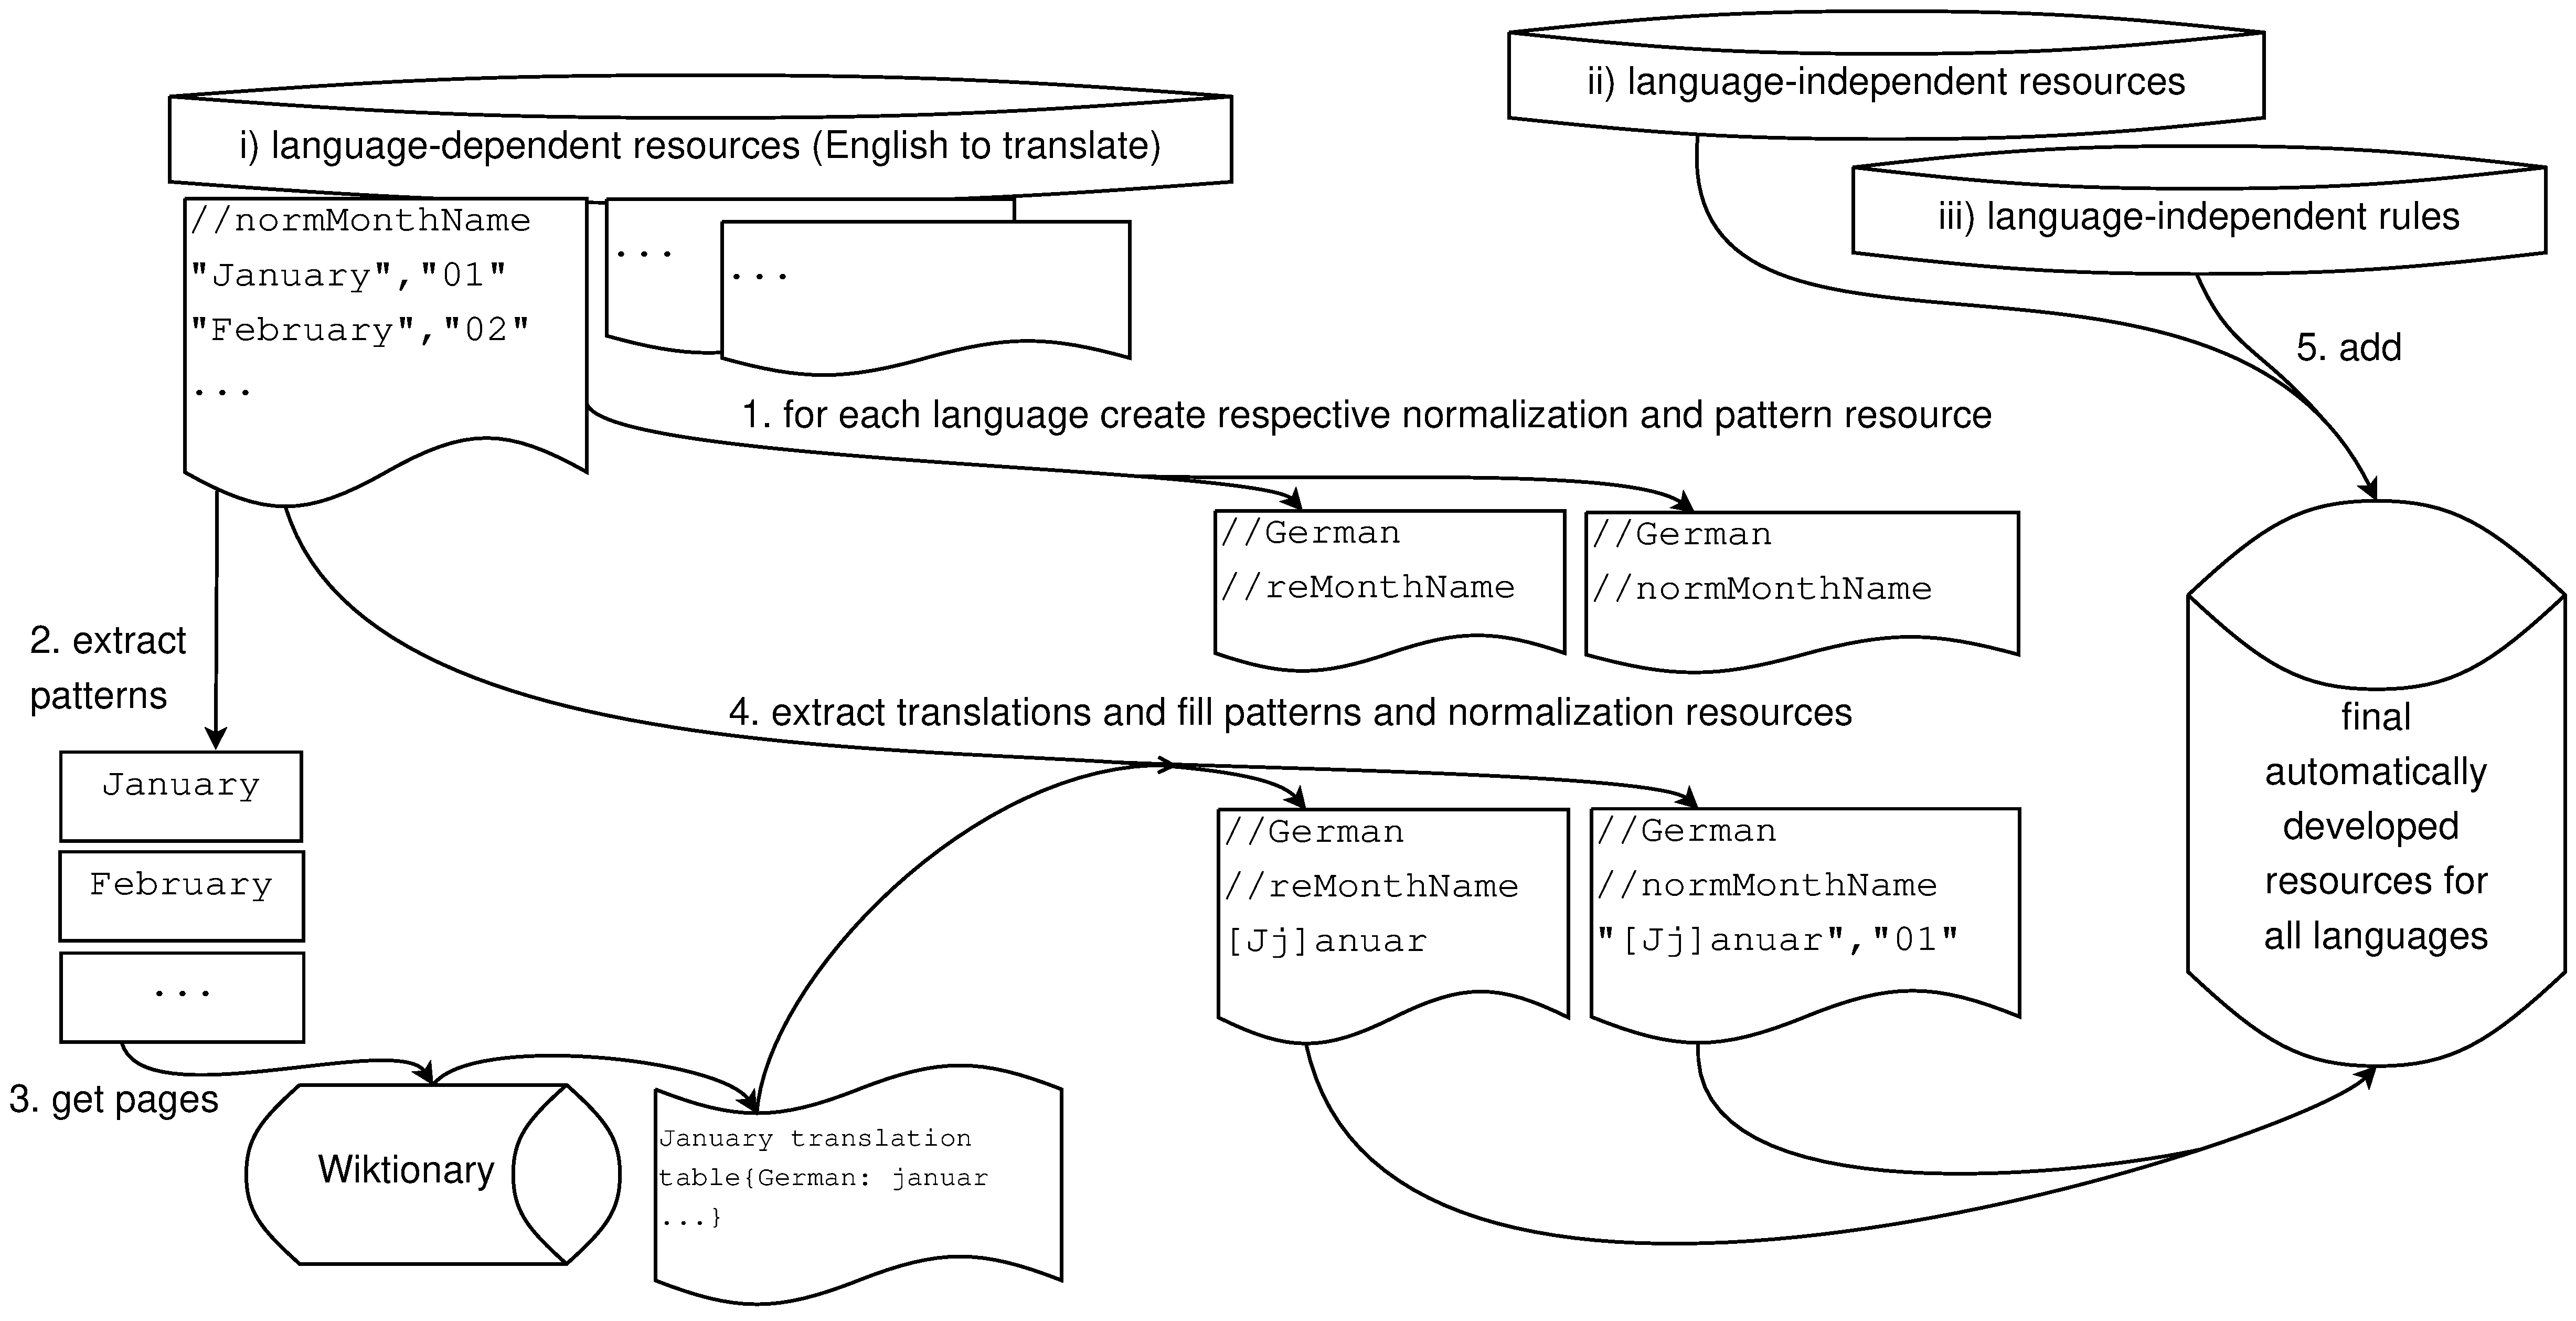
\includegraphics[width=14cm]{Graphics/ht-multilingual}
	\caption{Overview of Mutlilingual HeidelTime Model - adapted from \cite{DBLP:conf/emnlp/StrotgenG15}.}
	\label{figure:3d}
\end{figure}



\section{Multilingual HeidelTime Model Issues} \label{improved-multilingual-ht-model}
The Multilingual HeidelTime Model mentioned in the previous section, allowed HeidelTime to tag documents in many languages that had never been addressed before. These automatically developed resources can be used for baseline temporal tagging or can be a simple starting point to extend them to manual ones for any language. However, it had few shortcomings which we aim to address in this thesis: 

\begin{enumerate}[i.]
	\item Inflection was disregarded for morphologically rich languages in pattern and normalization resources.
	\item Unsegmented languages were not handled by the simplified language independent rules used by all languages.
	\item All languages used the same simplified langauge independent rules, ignoring intricacies of different languages and how temporal expressions might appear in them.
	\item Though not an issue with HeidelTime multilingual model in itself, tagging performance for the languages that lack temporal corpora was not evaluated or analysed.
\end{enumerate}

Now we discuss each of these issues in detail.

\subsection{Disregards Inflections}

The Multilingual HeidelTime model did not take into account the inflections of words for morphologically rich languages such as Polish, Finnish, Turkish, etc. For instance, at present, only translation in the pattern resource reMonthName for Finnish translation of January is [Tt]ammikuu., as shown in the listing below:\\

%\begin{figure}[H]
%	\centering
%	\includegraphics[width=8cm]{fi-reMonthName-ht-221}
%	\caption{reMonthName for Finnish language - using Multilingual HeidelTime Model }
%	\label{figure:3e}
%\end{figure}

\begin{minipage}{\linewidth}
\lstset{caption={reMonthName for Finnish language - using Multilingual HeidelTime Model - version 2.2.1.}, label={listing:3-fi-reMonthName-ht-221}}
\begin{lstlisting}
// english: "January","01"
[Tt]ammikuu
// english: "February","02"
[Hh]elmikuu
// english: "March","03"
[Mm]aaliskuu
// english: "April","04"
[Hh]uhtikuu
// english: "May","05"
[Tt]oukokuu
// ...
\end{lstlisting}
\end{minipage}


While total number of inflections for the Finnish word ``Tammikuu" are around 30, as shown in the Table \ref{table:1f} (page~\pageref{table:1f}). Having all the inflections for this word present in the resource reMonthName for Finnish will allow the rules to extract more temporal expressions. This is the first point we aim to address in this thesis.

\subsection{Ignores Unsegmented Languages}
The Multilingual HeidelTime model used same language independent rules for all languages, as mentioned in Subsection \ref{res-ir} item \ref{res-lir}. As the delimiter used in extraction part of these language independent rules is a space character, it leads to potentially missed extractions in languages that do not have whitespace tokenization between words, such as Thai and Japanese. Addressing rules resources for such languages would also be beneficial. This is the second point we aim to address in the thesis.

\subsection{No Language-specific Rules}
This issue is also related to the same language independent rules for all languages. We aim to learn some frequent temporal patterns as rules for each language and enrich the language independent rules with learned language-specific rules.

There are four types of rules in the language independent rules, i.e., date, duration, set and time, where each type of the rule corresponds to the four values the `type' property of TimeML TIMEX3 tag can take (TimeML is discussed in Subsection \ref{ss2as:timeml}, page \pageref{ss2as:timeml}).

We discuss the four types of language independent rules below:
\begin{enumerate}[i.]
	\item \textbf{Date rules:} The date rules resource file has rules to extract historic dates, complete dates, dates missing year information, names of days and expressions such as `since 1999', etc.
	\item \textbf{Duration rules:} The duration rules resource file has rules to extract temporal expressions such as `two years', `two months', `2 days', etc.  
	\item \textbf{Set rules} The set rules resource file has rules to extract temporal expressions such as `every year', `every month', `every July', etc.
	\item \textbf{Time rules} The time rules resource file has rules to extract temporal expressions such as `morning', `monday morning', `tomorrow morning', `next evening', etc.
\end{enumerate}

As the rules are language independent, some rules are written twice with alternating order of contributing rePattern files in them. For instance, the time rule to extract temporal expressions such as `tomorrow morning' has two rules. The extraction parts of these two rules are \framebox{\%rePartOfDay \%reDateWord} and \framebox{\%reDateWord \%rePartOfDay}. This is done as in some languages rePartOfDay might appear before reDateWord in such time temporal expressions. The two complete rules are given in the Listing \ref{listing:3-lirules} below, with rule name `time\_r1d' and `time\_r1e'.

Moreover, in date rules resource of the language independent rules, only year extraction rule is not present because there is a chance it can detect false positives, i.e., the four digits that do not represent actual year.

In the following listing, we list some of the language independent rules from each of the four types (date, duration, set and time). The comments above the rules give sample temporal expressions in English that can be extracted by respective rules. \\

\begin{minipage}{\linewidth}
\lstset{caption={Some sample language independent rules.}, label={listing:3-lirules}}
\begin{lstlisting}
// r3a: March 30, 2000
// r3b: March 30
RULENAME="date_r3a",EXTRACTION="%reMonthName %reDayNumber,? %reYear4Digit",NORM_VALUE="group(3)-%normMonthName(group(1))-%normDayNumber(group(2))"
RULENAME="date_r3b",EXTRACTION="%reMonthName %reDayNumber",NORM_VALUE="UNDEF-year-%normMonthName(group(1))-%normDayNumber(group(2))"

// r8a: since|until|in 2000
RULENAME="date_r8a",EXTRACTION="%reSinceEtAl %reYear4Digit",NORM_VALUE="group(2)",OFFSET="group(2)-group(2)"

// r2a: two years
RULENAME="duration_r2a",EXTRACTION="%reDayNumberWord4Duration %reUnit",NORM_VALUE="P%normDayNumberWord4Duration(group(1))%normUnit4Duration(group(2))"

// set_r1b: every Monday, each Sunday
RULENAME="set_r1b",EXTRACTION="%reEachEvery %reWeekday",NORM_VALUE="XXXX-WXX-%normDayInWeek(group(2))",NORM_QUANT="%UPPERCASE%(group(1))",NORM_FREQ="1W"

// r1a: morning
RULENAME="time_r1a",EXTRACTION="%rePartOfDay",NORM_VALUE="UNDEF-this-dayT%normPartOfDay(group(1))"

// time_r1d: morning tomorrow
// time_r1e: tomorrow morning 
RULENAME="time_r1d",EXTRACTION="%rePartOfDay %reDateWord",NORM_VALUE="%normDateWord(group(2))T%normPartOfDay(group(1))"
RULENAME="time_r1e",EXTRACTION="%reDateWord %rePartOfDay",NORM_VALUE="%normDateWord(group(1))T%normPartOfDay(group(2))"
\end{lstlisting}
\end{minipage}

Adding some language specific rules to the language independent rules for respective languages can further improve temporal tagging quality of HeidelTime. For instance, a rule that can extract only year temporal expressions, or the most frequently occurring order of complete date for different languages can be beneficial. We aim to learn some language specific rules for different languages, and enrich the language independent rules with those learned rules. This is the third point we aim to address in the thesis.

\subsection{Analysing Language Lacking Temporal Corpora} \label{the-chapter-3-alltc}
Though not an issue with HeidelTime resources, we aim to evaluate the languages that lack temporal corpora using Wikipedia dumps. These analysis results will be an important way to compare performance of the resources we create versus the initial ones, as there are no corpus available for most of the languages.

As Wikipedia dumps are not temporally annotated so there is no way to compute evaluation measures such as precision, recall or f1 score of extraction and normalization, unless we manually tag a subset of the dumps, which is impossible to do for all languages as it requires language experts and creating temporal corpora for even one language is very time and labour intensive. Doing analysis using Wikipedia dumps with different versions of HeidelTime resources can be a meaningful way of comparison between initial and the new resources. This is the fourth point we aim to address in the thesis.

